\Chapter{Következtetések és jövőbeli tervek}

A fejezet az alkalmazás helyét, későbbi jövőjét vetíti előre. Először az elért eredmények rövid értékelését láthatjuk, majd ötlet szintjén felsorolásra kerülnek azok az elemek, amelyek hosszabb távon sikeressé tehetnek egy ilyen alkalmazást.

\Section{Eredmények és következtetések}

Az eddig implementált, előbb felsorolt funkciók, elsőre jól hangzanak és bele is eshetünk abba a csapdába, hogy úgy gondolhatjuk ez elég is ahhoz, hogy rengeteg lelkes felhasználót gyűjtsünk és a sok általános iskolás mostantól imádnia fogja, ha közeleg egy adott dolgozat. Nyilván ez nem igaz, hisz ez nem ennyire egyszerű. Nem elég az, hogy pontokat, rangsorokat és kitűzőket rakunk bele egy koncepcióba és bízunk benne, hogy attól az garantáltan sokkal jobb lesz. Legalábbis hosszú távon, nagy hatást, biztos nem fog gyakorolni ránk. \newline

Azt is fontos lehet megérteni, hogy attól, hogy valamit máshogy hívunk nem jelenti azt, hogy az elvégzendő feladat attól jobb is lesz. Ha az egyetemen a számkérést nem zárthelyinek hívnák, hanem küldetéseknek, attól még ugyan úgy azt éreznénk, hogy zárthelyit írunk bárki, bárhogy hívja. Úgy gondolom, hogy az átnevezés akkor lehet sikeres csak, ha a cselekedet sorozat amit tenni kell a sikerért, megváltozik. Emellett ha valamit játékosítani szeretnénk úgy, hogy az hosszútávon motiváló és érdekes maradjon akkor ahhoz még több elemet kéne belevinni. Ha csak visszatérünk a bevezetésnél említett Duolingo-ra, azt például 2012 óta fejlesztik, ma már több mint 200 alkalmazottal. Tehát ez több éves munka eredménye, hogy egy ilyen játékos környezetet kialakítsunk és felépítsünk hiszen sok összetevő játszik számot benne. \newline

Az, hogy mik ezek az összetevők, azt Yu-Kai Chou korábban említett könyvében megfogalmazta \cite{actionablegamification}. Megfigyelte, hogy a játékok nagy részét ugyan az a 8 hajtóerő (\textit{core drives}) írja le. Ezek azok az elemek amelyek képesek a játékost lekötni és játékban tartani.

\begin{figure}[H]
    \centering
    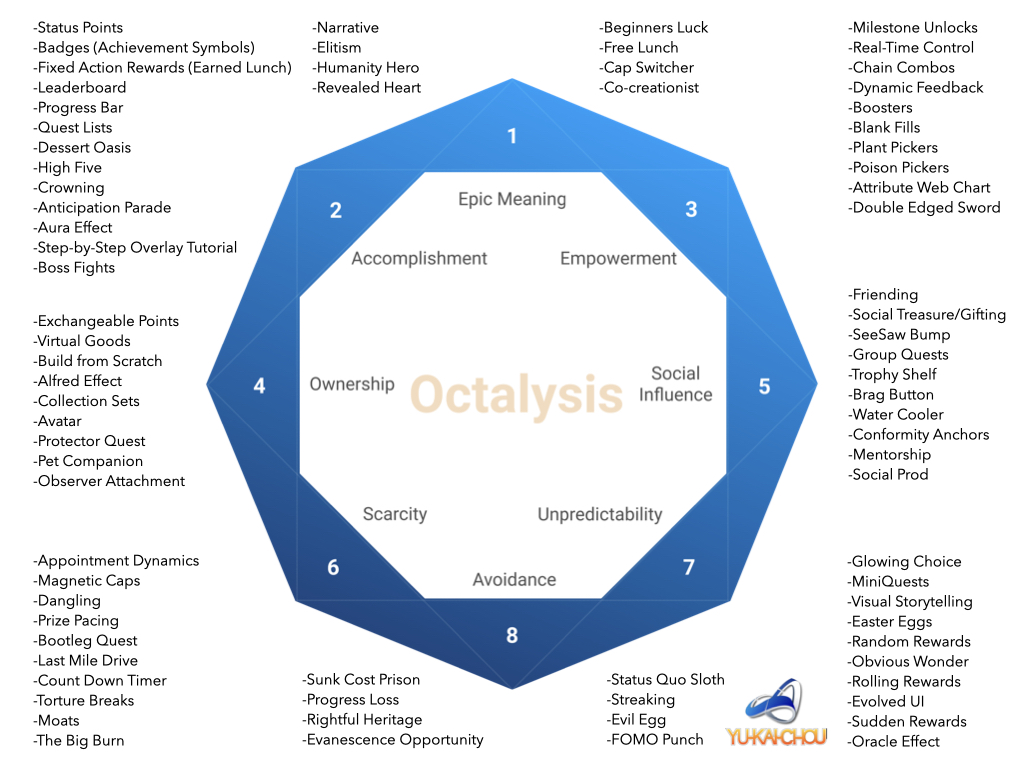
\includegraphics[width=\linewidth]{images/gamification-framework.jpg}
    \caption{Yu-Kai Chou oktalízis rendszere}
    \label{fig:gamification-framework}
\end{figure}

Az oktalízis rendszer (\prettyref{fig:gamification-framework}. ábra) egybefoglalja és számszerűsíti ezeket a játékon belül megtalálható motivációs tényezőket. \newline

Itt 8 hajtőerőt sorol fel, amik egy rendszert játékossá tesznek. Így egyben látható, hogy ez rengeteg összetevő és funkció sokasága ami egy felhasználót be tud szippantani. Tehát egy komoly rendszer fejlesztése nem kevés időt és energiát igényel. Viszont azokat amiket nekem, sikerült beleraknom azokat felsorolnám.

\begin{itemize}
    \item {Teljesítmény (Accomplishment)}
          \begin{addmargin}[\parindent]{0pt}
              Ezek azok a dolgok amik hajtanak minket abba az irányba, hogy kihívásokkal szembenézzünk és teljesítsük őket. Ilyen a pontszerzés, szintlépés és tesztek végén lévő rangsor.
          \end{addmargin}
    \item {Kiszámíthatatlanság (Unpredictability)}
          \begin{addmargin}[\parindent]{0pt}
              Ez abban segít a felhasználó izgatott legyen az oldal használata közben. Nyilván ez tulajdonság adja magát hiszen minden tesztet csak a készítője ismer.
          \end{addmargin}
    \item {Társadalmi befolyás (Social Influence)}
          \begin{addmargin}[\parindent]{0pt}
              Ha meglátjuk, hogy az egyik barátunk nagyon jól teljesített egy teszten, akkor késztetést érzünk arra mi is, hogy ugyan úgy elérjük. Ezért is van teszt végén rangsorolás.
          \end{addmargin}
    \item {Fejlődés (Empowerment)}
          \begin{addmargin}[\parindent]{0pt}
            Az embereknek látniuk kell munkájuk eredményét, visszajelzéseket kell kapniuk. Ezt a fejlődést a szintek indikálják.
          \end{addmargin}
    \item {Magasabb jelentés (Epic meaning)}
          \begin{addmargin}[\parindent]{0pt}
              A magasabb jelentés az amikor valaki olyat teszi ami nála nagyobb, egy magasabb érdeket elégít ki. Ez a mi esetünkben ez lehet az, hogy valaki elvégezze az egyetemet vagy érettségit szerezzen. Ahhoz, hogy ez valóra váljon, a tesztjeinek sikereseknek kell lennie. Ez ösztönözheti az oldal használatára.
          \end{addmargin}
\end{itemize}

\Section{Jövőbeli tervek}

Az alkalmazásban egy teszt készítéséhez szükséges alap funkciók meg vannak már valósítva, mindazonáltal még rengeteg lehetőség rejlik ebben a szoftverben. Az alábbiakat lehetne még hozzáadni:

\subsubsection{Bolt}
Az alkalmazáson belül lehetne kitalálni saját pénznemet, vagy akár a pontjaiddal is fel lehetne fizetni és különböző előnyöket lehetne ebből venni. Ezek az előnyök minden kérdésnél feljönnének és lehetne őket aktiválni egyszer. Ilyen előny lehet például, hogy le lehet felezni a válaszokat, lehessen növel az időt vagy akár, hogy plusz xp-t kapjunk egy tesztre.

\subsubsection{Kitűzőket létrehozni jutalmazás miatt}
Lehetne kitűzőket gyűjteni, ebből olyanok lehetne elérni, mint például tesztben 5 vagy 10 kérdésre egymás utána helyes választ adott a kitöltő, több mint 3 tesztben 500 feletti XP-t ért el vagy 3 kérdésre gyorsan adott jó választ.

\subsubsection{Tesztek összekeverése}
Az online tesztkitöltések egyik hátránya, hogy könnyebb csalni kitöltés során. Ennek megnehezítésének egyik módja az lehetne, hogy a kérdések véletlenszerű sorrendben jönnek fel mindenkinél.

\subsubsection{Avatár készítés}
A tulajdonjog és birtoklás is ugyan úgy motiválja a felhasználót, mert úgy érzik, hogy valamit birtokolnak vagy irányítanak. Amikor egy személy valamit a tulajdonának érez valamivel szemben, akkor automatikusan növelni és fejleszteni akarja azt. Ezenkívül, ha egy személy sok időt tölt profilja vagy avatárjának testre szabásával, automatikusan nagyobb felelősséget érez iránta. Emiatt bele lehetne tenni a regisztrációhoz egy avatár készítő felületet, ahol magukat vagy akár egy kitalált karaktert, hozhat létre az új felhasználó és magáénak érezheti a profilját. Ezeket az avatárok megjelennének a főoldalon és a ranglistán az eredmények mellett.

\subsubsection{Osztályok, csoportok létrehozása}
Az oldal használatához a kötődést nagyban megnövelhetné, ha közösségeket lehetne létrehozni benne. Ennek kapcsán arra gondolok, hogy a tesztkitöltők között általában van valamilyen kapcsolat, ez döntő többségben iskolához köthető kapcsolat, például egy osztályba járnak vagy egy szakon vannak az egyetemen. Emiatt hasznos lenne, ha lehetne ilyen csoportokat létrehozni, ahol esetleg kérdéseket tudnának feltenni a tanárnak vagy átbeszélni a tesztel kapcsolatos dolgokat. Így motiválnák egymást a tanulásra és jobban teljesítenének. Valamint a tanároknak is nagy segítség lehetne, mivel teszt készítésnél a kitöltőknél nem egyesével kéne beírniuk az email címeket, hanem mondjuk kiválaszthatná a csoportot név alapján és hozzá rendelhetné a csoport összes tagjához.

\subsubsection{Felhasználók profiljának megtekintése}
Lehetne felhasználói profilokat is megtekinteni. Itt listázva lenne a közelmúltban szerzett eredmények, jelvényei vagy, hogy milyen csoportoknak a tagja. Ezáltal növelné a versenyszellemet a felhasználók között, mivel láthatnák, ki mennyi pontot szerzett mostanában.
